% Options for packages loaded elsewhere
\PassOptionsToPackage{unicode}{hyperref}
\PassOptionsToPackage{hyphens}{url}
\PassOptionsToPackage{dvipsnames,svgnames,x11names}{xcolor}
%
\documentclass[
  letterpaper,
  DIV=11,
  numbers=noendperiod]{scrartcl}

\usepackage{amsmath,amssymb}
\usepackage{iftex}
\ifPDFTeX
  \usepackage[T1]{fontenc}
  \usepackage[utf8]{inputenc}
  \usepackage{textcomp} % provide euro and other symbols
\else % if luatex or xetex
  \usepackage{unicode-math}
  \defaultfontfeatures{Scale=MatchLowercase}
  \defaultfontfeatures[\rmfamily]{Ligatures=TeX,Scale=1}
\fi
\usepackage{lmodern}
\ifPDFTeX\else  
    % xetex/luatex font selection
\fi
% Use upquote if available, for straight quotes in verbatim environments
\IfFileExists{upquote.sty}{\usepackage{upquote}}{}
\IfFileExists{microtype.sty}{% use microtype if available
  \usepackage[]{microtype}
  \UseMicrotypeSet[protrusion]{basicmath} % disable protrusion for tt fonts
}{}
\makeatletter
\@ifundefined{KOMAClassName}{% if non-KOMA class
  \IfFileExists{parskip.sty}{%
    \usepackage{parskip}
  }{% else
    \setlength{\parindent}{0pt}
    \setlength{\parskip}{6pt plus 2pt minus 1pt}}
}{% if KOMA class
  \KOMAoptions{parskip=half}}
\makeatother
\usepackage{xcolor}
\setlength{\emergencystretch}{3em} % prevent overfull lines
\setcounter{secnumdepth}{-\maxdimen} % remove section numbering
% Make \paragraph and \subparagraph free-standing
\makeatletter
\ifx\paragraph\undefined\else
  \let\oldparagraph\paragraph
  \renewcommand{\paragraph}{
    \@ifstar
      \xxxParagraphStar
      \xxxParagraphNoStar
  }
  \newcommand{\xxxParagraphStar}[1]{\oldparagraph*{#1}\mbox{}}
  \newcommand{\xxxParagraphNoStar}[1]{\oldparagraph{#1}\mbox{}}
\fi
\ifx\subparagraph\undefined\else
  \let\oldsubparagraph\subparagraph
  \renewcommand{\subparagraph}{
    \@ifstar
      \xxxSubParagraphStar
      \xxxSubParagraphNoStar
  }
  \newcommand{\xxxSubParagraphStar}[1]{\oldsubparagraph*{#1}\mbox{}}
  \newcommand{\xxxSubParagraphNoStar}[1]{\oldsubparagraph{#1}\mbox{}}
\fi
\makeatother

\usepackage{color}
\usepackage{fancyvrb}
\newcommand{\VerbBar}{|}
\newcommand{\VERB}{\Verb[commandchars=\\\{\}]}
\DefineVerbatimEnvironment{Highlighting}{Verbatim}{commandchars=\\\{\}}
% Add ',fontsize=\small' for more characters per line
\usepackage{framed}
\definecolor{shadecolor}{RGB}{241,243,245}
\newenvironment{Shaded}{\begin{snugshade}}{\end{snugshade}}
\newcommand{\AlertTok}[1]{\textcolor[rgb]{0.68,0.00,0.00}{#1}}
\newcommand{\AnnotationTok}[1]{\textcolor[rgb]{0.37,0.37,0.37}{#1}}
\newcommand{\AttributeTok}[1]{\textcolor[rgb]{0.40,0.45,0.13}{#1}}
\newcommand{\BaseNTok}[1]{\textcolor[rgb]{0.68,0.00,0.00}{#1}}
\newcommand{\BuiltInTok}[1]{\textcolor[rgb]{0.00,0.23,0.31}{#1}}
\newcommand{\CharTok}[1]{\textcolor[rgb]{0.13,0.47,0.30}{#1}}
\newcommand{\CommentTok}[1]{\textcolor[rgb]{0.37,0.37,0.37}{#1}}
\newcommand{\CommentVarTok}[1]{\textcolor[rgb]{0.37,0.37,0.37}{\textit{#1}}}
\newcommand{\ConstantTok}[1]{\textcolor[rgb]{0.56,0.35,0.01}{#1}}
\newcommand{\ControlFlowTok}[1]{\textcolor[rgb]{0.00,0.23,0.31}{\textbf{#1}}}
\newcommand{\DataTypeTok}[1]{\textcolor[rgb]{0.68,0.00,0.00}{#1}}
\newcommand{\DecValTok}[1]{\textcolor[rgb]{0.68,0.00,0.00}{#1}}
\newcommand{\DocumentationTok}[1]{\textcolor[rgb]{0.37,0.37,0.37}{\textit{#1}}}
\newcommand{\ErrorTok}[1]{\textcolor[rgb]{0.68,0.00,0.00}{#1}}
\newcommand{\ExtensionTok}[1]{\textcolor[rgb]{0.00,0.23,0.31}{#1}}
\newcommand{\FloatTok}[1]{\textcolor[rgb]{0.68,0.00,0.00}{#1}}
\newcommand{\FunctionTok}[1]{\textcolor[rgb]{0.28,0.35,0.67}{#1}}
\newcommand{\ImportTok}[1]{\textcolor[rgb]{0.00,0.46,0.62}{#1}}
\newcommand{\InformationTok}[1]{\textcolor[rgb]{0.37,0.37,0.37}{#1}}
\newcommand{\KeywordTok}[1]{\textcolor[rgb]{0.00,0.23,0.31}{\textbf{#1}}}
\newcommand{\NormalTok}[1]{\textcolor[rgb]{0.00,0.23,0.31}{#1}}
\newcommand{\OperatorTok}[1]{\textcolor[rgb]{0.37,0.37,0.37}{#1}}
\newcommand{\OtherTok}[1]{\textcolor[rgb]{0.00,0.23,0.31}{#1}}
\newcommand{\PreprocessorTok}[1]{\textcolor[rgb]{0.68,0.00,0.00}{#1}}
\newcommand{\RegionMarkerTok}[1]{\textcolor[rgb]{0.00,0.23,0.31}{#1}}
\newcommand{\SpecialCharTok}[1]{\textcolor[rgb]{0.37,0.37,0.37}{#1}}
\newcommand{\SpecialStringTok}[1]{\textcolor[rgb]{0.13,0.47,0.30}{#1}}
\newcommand{\StringTok}[1]{\textcolor[rgb]{0.13,0.47,0.30}{#1}}
\newcommand{\VariableTok}[1]{\textcolor[rgb]{0.07,0.07,0.07}{#1}}
\newcommand{\VerbatimStringTok}[1]{\textcolor[rgb]{0.13,0.47,0.30}{#1}}
\newcommand{\WarningTok}[1]{\textcolor[rgb]{0.37,0.37,0.37}{\textit{#1}}}

\providecommand{\tightlist}{%
  \setlength{\itemsep}{0pt}\setlength{\parskip}{0pt}}\usepackage{longtable,booktabs,array}
\usepackage{calc} % for calculating minipage widths
% Correct order of tables after \paragraph or \subparagraph
\usepackage{etoolbox}
\makeatletter
\patchcmd\longtable{\par}{\if@noskipsec\mbox{}\fi\par}{}{}
\makeatother
% Allow footnotes in longtable head/foot
\IfFileExists{footnotehyper.sty}{\usepackage{footnotehyper}}{\usepackage{footnote}}
\makesavenoteenv{longtable}
\usepackage{graphicx}
\makeatletter
\def\maxwidth{\ifdim\Gin@nat@width>\linewidth\linewidth\else\Gin@nat@width\fi}
\def\maxheight{\ifdim\Gin@nat@height>\textheight\textheight\else\Gin@nat@height\fi}
\makeatother
% Scale images if necessary, so that they will not overflow the page
% margins by default, and it is still possible to overwrite the defaults
% using explicit options in \includegraphics[width, height, ...]{}
\setkeys{Gin}{width=\maxwidth,height=\maxheight,keepaspectratio}
% Set default figure placement to htbp
\makeatletter
\def\fps@figure{htbp}
\makeatother

\KOMAoption{captions}{tableheading}
\makeatletter
\@ifpackageloaded{caption}{}{\usepackage{caption}}
\AtBeginDocument{%
\ifdefined\contentsname
  \renewcommand*\contentsname{Índice}
\else
  \newcommand\contentsname{Índice}
\fi
\ifdefined\listfigurename
  \renewcommand*\listfigurename{Lista de Figuras}
\else
  \newcommand\listfigurename{Lista de Figuras}
\fi
\ifdefined\listtablename
  \renewcommand*\listtablename{Lista de Tabelas}
\else
  \newcommand\listtablename{Lista de Tabelas}
\fi
\ifdefined\figurename
  \renewcommand*\figurename{Figura}
\else
  \newcommand\figurename{Figura}
\fi
\ifdefined\tablename
  \renewcommand*\tablename{Tabela}
\else
  \newcommand\tablename{Tabela}
\fi
}
\@ifpackageloaded{float}{}{\usepackage{float}}
\floatstyle{ruled}
\@ifundefined{c@chapter}{\newfloat{codelisting}{h}{lop}}{\newfloat{codelisting}{h}{lop}[chapter]}
\floatname{codelisting}{Listagem}
\newcommand*\listoflistings{\listof{codelisting}{Lista de Listagens}}
\makeatother
\makeatletter
\makeatother
\makeatletter
\@ifpackageloaded{caption}{}{\usepackage{caption}}
\@ifpackageloaded{subcaption}{}{\usepackage{subcaption}}
\makeatother

\ifLuaTeX
\usepackage[bidi=basic]{babel}
\else
\usepackage[bidi=default]{babel}
\fi
\babelprovide[main,import]{portuguese}
% get rid of language-specific shorthands (see #6817):
\let\LanguageShortHands\languageshorthands
\def\languageshorthands#1{}
\ifLuaTeX
  \usepackage{selnolig}  % disable illegal ligatures
\fi
\usepackage{bookmark}

\IfFileExists{xurl.sty}{\usepackage{xurl}}{} % add URL line breaks if available
\urlstyle{same} % disable monospaced font for URLs
\hypersetup{
  pdftitle={Regressão Linear Múltipla},
  pdfauthor={Larysa Mendes, Vitória Maria, Welly Remígio},
  pdflang={pt},
  colorlinks=true,
  linkcolor={blue},
  filecolor={Maroon},
  citecolor={Blue},
  urlcolor={Blue},
  pdfcreator={LaTeX via pandoc}}


\title{Regressão Linear Múltipla}
\author{Larysa Mendes, Vitória Maria, Welly Remígio}
\date{2024-10-02}

\begin{document}
\maketitle


\begin{Shaded}
\begin{Highlighting}[]
\CommentTok{\# Setup para o relatório Quarto}

\NormalTok{knitr}\SpecialCharTok{::}\NormalTok{opts\_chunk}\SpecialCharTok{$}\FunctionTok{set}\NormalTok{(}\AttributeTok{echo =} \ConstantTok{TRUE}\NormalTok{, }\AttributeTok{message =} \ConstantTok{FALSE}\NormalTok{, }\AttributeTok{warning =} \ConstantTok{FALSE}\NormalTok{)}

\CommentTok{\# Definindo o espelho do CRAN}
\FunctionTok{options}\NormalTok{(}\AttributeTok{repos =} \FunctionTok{c}\NormalTok{(}\AttributeTok{CRAN =} \StringTok{"https://cloud.r{-}project.org/"}\NormalTok{))}
\end{Highlighting}
\end{Shaded}

\section{Introdução}\label{introduuxe7uxe3o}

Este relatório tem por objetivo ajustar um modelo de regressão linear
múltiplo com o intuito de investigar a influência de determinadas
características associadas a vendas de cadeirinhas de carro para
crianças e diversos fatores que podem influenciar essas vendas.

Neste contexto a regressão será realizada sobre base de dados
\texttt{Carseats}, que trata das vendas de cadeirinhas de carro para
crianças (Child Car Seats) em diferentes locais. Essa base está na
biblioteca ISLR (An Introduction to Statistical Learning with
Applications in R) que é um pacote em R que acompanha o famoso livro
``An Introduction to Statistical Learning'' (ISLR). Ela contém vários
conjuntos de dados usados para demonstrar técnicas de aprendizado
estatístico e machine learning. Essa base de dados contém onze
variáveis, sendo três destas quanlitativas, as demais são medidas
quantitativas.

\section{Os dados}\label{os-dados}

É possível baixar os dados do livro
\href{https://www.statlearning.com/}{An Introduction to Statistical
Learning with applications in R}, mas o pacote \texttt{ISLR} pode ser
baixado diretamente do \emph{R}, para acessar a base de dados,
\texttt{Carseats}.

\begin{Shaded}
\begin{Highlighting}[]
\FunctionTok{install.packages}\NormalTok{(}\StringTok{"ISLR"}\NormalTok{, }\AttributeTok{quiet=}\ConstantTok{TRUE}\NormalTok{) }\CommentTok{\#instalando pacote}
\end{Highlighting}
\end{Shaded}

\begin{verbatim}
package 'ISLR' successfully unpacked and MD5 sums checked
\end{verbatim}

\begin{Shaded}
\begin{Highlighting}[]
\FunctionTok{library}\NormalTok{(ISLR) }\CommentTok{\#chamando pacote}

\FunctionTok{setwd}\NormalTok{(}\StringTok{"C:}\SpecialCharTok{\textbackslash{}\textbackslash{}}\StringTok{Users}\SpecialCharTok{\textbackslash{}\textbackslash{}}\StringTok{Notebook}\SpecialCharTok{\textbackslash{}\textbackslash{}}\StringTok{Documents}\SpecialCharTok{\textbackslash{}\textbackslash{}}\StringTok{Relatorio\_Estatistica"}\NormalTok{)}
\FunctionTok{write.table}\NormalTok{(Carseats , }\AttributeTok{file=}\StringTok{"nome\_do\_arquivo.csv"}\NormalTok{, }\AttributeTok{sep=}\StringTok{";"}\NormalTok{, }\AttributeTok{dec=}\StringTok{","}\NormalTok{) }\CommentTok{\#criando arquivo .csv no local de }
\CommentTok{\#help("Carseats") \#descrição das variáveis}
\CommentTok{\#glimpse(Carseats)}
\end{Highlighting}
\end{Shaded}

Descrição da Base de Dados: Número de observações: 400 Variável
Resposta: - \texttt{Sales}: Vendas de cadeirinhas de carro em diferentes
locais. (Milhares de unidades)

Variáveis Explicativas: - \texttt{CompPrice}: Preço da cadeirinha na
loja concorrente. (em dólares).\\
- \texttt{Income}: Renda média dos consumidores naquela região. (em
milhares de dólares).\\
- \texttt{Advertising}: Valor gasto em publicidade para aquela região
(em milhares de dólares).\\
- \texttt{Population}: População da região. (em milhares).\\
- \texttt{Price}: Preço da cadeirinha de carro na loja.(em dólares).\\
- \texttt{ShelveLoc}: Qualidade da localização da prateleira na loja.
(``Good'', ``Medium'', ``Bad'').\\
- \texttt{Age}: Idade média da população na região. (em anos).\\
- \texttt{Education}: Nível médio de educação da população na região.(em
anos).\\
- \texttt{Urban}: Um fator que indica se a região é urbana. (``Yes'' ou
``No'').\\
- \texttt{US}: Um fator que indica se a loja está nos EUA. (``Yes'' ou
``No'').

\subsection{Análise exploratória dos
dados}\label{anuxe1lise-exploratuxf3ria-dos-dados}

\begin{Shaded}
\begin{Highlighting}[]
\FunctionTok{library}\NormalTok{(skimr)}

\NormalTok{dados }\OtherTok{\textless{}{-}}\NormalTok{ Carseats}

\FunctionTok{skim}\NormalTok{(dados)}
\end{Highlighting}
\end{Shaded}

\begin{longtable}[]{@{}ll@{}}
\caption{Data summary}\tabularnewline
\toprule\noalign{}
\endfirsthead
\endhead
\bottomrule\noalign{}
\endlastfoot
Name & dados \\
Number of rows & 400 \\
Number of columns & 11 \\
\_\_\_\_\_\_\_\_\_\_\_\_\_\_\_\_\_\_\_\_\_\_\_ & \\
Column type frequency: & \\
factor & 3 \\
numeric & 8 \\
\_\_\_\_\_\_\_\_\_\_\_\_\_\_\_\_\_\_\_\_\_\_\_\_ & \\
Group variables & None \\
\end{longtable}

\textbf{Variable type: factor}

\begin{longtable}[]{@{}
  >{\raggedright\arraybackslash}p{(\columnwidth - 10\tabcolsep) * \real{0.1707}}
  >{\raggedleft\arraybackslash}p{(\columnwidth - 10\tabcolsep) * \real{0.1220}}
  >{\raggedleft\arraybackslash}p{(\columnwidth - 10\tabcolsep) * \real{0.1707}}
  >{\raggedright\arraybackslash}p{(\columnwidth - 10\tabcolsep) * \real{0.0976}}
  >{\raggedleft\arraybackslash}p{(\columnwidth - 10\tabcolsep) * \real{0.1098}}
  >{\raggedright\arraybackslash}p{(\columnwidth - 10\tabcolsep) * \real{0.3293}}@{}}
\toprule\noalign{}
\begin{minipage}[b]{\linewidth}\raggedright
skim\_variable
\end{minipage} & \begin{minipage}[b]{\linewidth}\raggedleft
n\_missing
\end{minipage} & \begin{minipage}[b]{\linewidth}\raggedleft
complete\_rate
\end{minipage} & \begin{minipage}[b]{\linewidth}\raggedright
ordered
\end{minipage} & \begin{minipage}[b]{\linewidth}\raggedleft
n\_unique
\end{minipage} & \begin{minipage}[b]{\linewidth}\raggedright
top\_counts
\end{minipage} \\
\midrule\noalign{}
\endhead
\bottomrule\noalign{}
\endlastfoot
ShelveLoc & 0 & 1 & FALSE & 3 & Med: 219, Bad: 96, Goo: 85 \\
Urban & 0 & 1 & FALSE & 2 & Yes: 282, No: 118 \\
US & 0 & 1 & FALSE & 2 & Yes: 258, No: 142 \\
\end{longtable}

\textbf{Variable type: numeric}

\begin{longtable}[]{@{}
  >{\raggedright\arraybackslash}p{(\columnwidth - 20\tabcolsep) * \real{0.1573}}
  >{\raggedleft\arraybackslash}p{(\columnwidth - 20\tabcolsep) * \real{0.1124}}
  >{\raggedleft\arraybackslash}p{(\columnwidth - 20\tabcolsep) * \real{0.1573}}
  >{\raggedleft\arraybackslash}p{(\columnwidth - 20\tabcolsep) * \real{0.0787}}
  >{\raggedleft\arraybackslash}p{(\columnwidth - 20\tabcolsep) * \real{0.0787}}
  >{\raggedleft\arraybackslash}p{(\columnwidth - 20\tabcolsep) * \real{0.0337}}
  >{\raggedleft\arraybackslash}p{(\columnwidth - 20\tabcolsep) * \real{0.0787}}
  >{\raggedleft\arraybackslash}p{(\columnwidth - 20\tabcolsep) * \real{0.0787}}
  >{\raggedleft\arraybackslash}p{(\columnwidth - 20\tabcolsep) * \real{0.0787}}
  >{\raggedleft\arraybackslash}p{(\columnwidth - 20\tabcolsep) * \real{0.0787}}
  >{\raggedright\arraybackslash}p{(\columnwidth - 20\tabcolsep) * \real{0.0674}}@{}}
\toprule\noalign{}
\begin{minipage}[b]{\linewidth}\raggedright
skim\_variable
\end{minipage} & \begin{minipage}[b]{\linewidth}\raggedleft
n\_missing
\end{minipage} & \begin{minipage}[b]{\linewidth}\raggedleft
complete\_rate
\end{minipage} & \begin{minipage}[b]{\linewidth}\raggedleft
mean
\end{minipage} & \begin{minipage}[b]{\linewidth}\raggedleft
sd
\end{minipage} & \begin{minipage}[b]{\linewidth}\raggedleft
p0
\end{minipage} & \begin{minipage}[b]{\linewidth}\raggedleft
p25
\end{minipage} & \begin{minipage}[b]{\linewidth}\raggedleft
p50
\end{minipage} & \begin{minipage}[b]{\linewidth}\raggedleft
p75
\end{minipage} & \begin{minipage}[b]{\linewidth}\raggedleft
p100
\end{minipage} & \begin{minipage}[b]{\linewidth}\raggedright
hist
\end{minipage} \\
\midrule\noalign{}
\endhead
\bottomrule\noalign{}
\endlastfoot
Sales & 0 & 1 & 7.50 & 2.82 & 0 & 5.39 & 7.49 & 9.32 & 16.27 & ▁▆▇▃▁ \\
CompPrice & 0 & 1 & 124.97 & 15.33 & 77 & 115.00 & 125.00 & 135.00 &
175.00 & ▁▅▇▃▁ \\
Income & 0 & 1 & 68.66 & 27.99 & 21 & 42.75 & 69.00 & 91.00 & 120.00 &
▇▆▇▆▅ \\
Advertising & 0 & 1 & 6.64 & 6.65 & 0 & 0.00 & 5.00 & 12.00 & 29.00 &
▇▃▃▁▁ \\
Population & 0 & 1 & 264.84 & 147.38 & 10 & 139.00 & 272.00 & 398.50 &
509.00 & ▇▇▇▇▇ \\
Price & 0 & 1 & 115.80 & 23.68 & 24 & 100.00 & 117.00 & 131.00 & 191.00
& ▁▂▇▆▁ \\
Age & 0 & 1 & 53.32 & 16.20 & 25 & 39.75 & 54.50 & 66.00 & 80.00 &
▇▆▇▇▇ \\
Education & 0 & 1 & 13.90 & 2.62 & 10 & 12.00 & 14.00 & 16.00 & 18.00 &
▇▇▃▇▇ \\
\end{longtable}

\subsubsection{Comentários:}\label{comentuxe1rios}

De acordo com a tabela é possível observar que não há ausência de dados.
\# INCOMPLETO

\subsubsection{Análise de Correlação}\label{sec-GGally}

\begin{Shaded}
\begin{Highlighting}[]
\FunctionTok{install.packages}\NormalTok{(}\StringTok{"GGally"}\NormalTok{, }\AttributeTok{quite=}\ConstantTok{TRUE}\NormalTok{)}
\end{Highlighting}
\end{Shaded}

\begin{verbatim}
package 'GGally' successfully unpacked and MD5 sums checked

The downloaded binary packages are in
    C:\Users\Notebook\AppData\Local\Temp\RtmpA3V7Vh\downloaded_packages
\end{verbatim}

\begin{Shaded}
\begin{Highlighting}[]
\FunctionTok{library}\NormalTok{(GGally)}\CommentTok{\# Pacote para função ggpairs}
\FunctionTok{library}\NormalTok{(ggplot2)}


\DocumentationTok{\#\#\# Multicolinearidade: r \textgreater{} 0.9 (ou 0.8)}

\NormalTok{graf1 }\OtherTok{\textless{}{-}} \FunctionTok{ggpairs}\NormalTok{(dados, }
                 \AttributeTok{columns =} \FunctionTok{c}\NormalTok{(}\StringTok{"Sales"}\NormalTok{, }\StringTok{"CompPrice"}\NormalTok{, }\StringTok{"Income"}\NormalTok{, }\StringTok{"Advertising"}\NormalTok{, }\StringTok{"Population"}\NormalTok{, }\StringTok{"Price"}\NormalTok{, }\StringTok{"Age"}\NormalTok{, }\StringTok{"Education"}\NormalTok{), }
\NormalTok{                 ggplot2}\SpecialCharTok{::}\FunctionTok{aes}\NormalTok{(}\AttributeTok{colour=}\NormalTok{US), }
                 \AttributeTok{upper =} \FunctionTok{list}\NormalTok{(}\AttributeTok{continuous =} \FunctionTok{wrap}\NormalTok{(}\StringTok{"cor"}\NormalTok{, }\AttributeTok{size =} \DecValTok{3}\NormalTok{)), }
                 \AttributeTok{lower =} \FunctionTok{list}\NormalTok{(}\AttributeTok{continuous =} \StringTok{"points"}\NormalTok{)) }\SpecialCharTok{+}            
  \FunctionTok{theme\_minimal}\NormalTok{() }\SpecialCharTok{+}                                              
  \FunctionTok{theme}\NormalTok{(}\AttributeTok{axis.text =} \FunctionTok{element\_text}\NormalTok{(}\AttributeTok{size =} \DecValTok{8}\NormalTok{),                      }
        \AttributeTok{legend.position =} \StringTok{"bottom"}\NormalTok{,                              }
        \AttributeTok{strip.text =} \FunctionTok{element\_text}\NormalTok{(}\AttributeTok{size =} \DecValTok{10}\NormalTok{))    }

\NormalTok{graf1}
\end{Highlighting}
\end{Shaded}

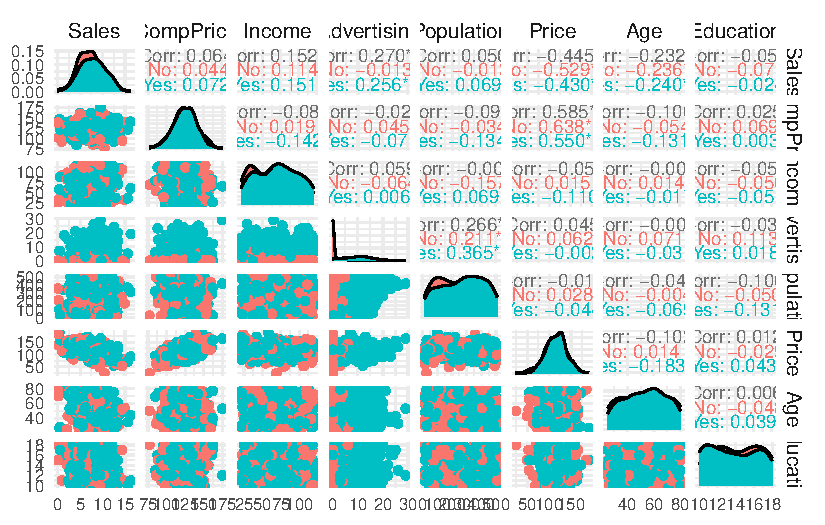
\includegraphics{teste_files/figure-pdf/unnamed-chunk-3-1.pdf}

\begin{Shaded}
\begin{Highlighting}[]
\CommentTok{\# Salvando o gráfico em .jpeg}
\FunctionTok{ggsave}\NormalTok{(}\StringTok{"Grafico\_dispersao\_carseats.jpeg"}\NormalTok{)}
\end{Highlighting}
\end{Shaded}

\paragraph{Comentários}\label{comentuxe1rios-1}

Com relação à análise de correlação é algo desejável observar altas
correlações das variáveis independentes com relação à variável
dependente que no presente caso é \texttt{Sales}.

Por outro lado, altas correlações entre as demais variáveis a serem
utilizadas como variáveis independentes nos dá indícios de que haverá
\textbf{problemas de multicolinearidade} ao ajustar o MRLM. \textbf{Como
regra geral} isto ocorre quando há \textbf{correlações} \(\geq 0.9\) ou
\(\geq 0.8\) \textbf{entre} as \textbf{variáveis preditoras}.

Dito isto, é possível observar que:

\begin{enumerate}
\def\labelenumi{\arabic{enumi})}
\tightlist
\item
  A variável dependente \texttt{Sales}:
\end{enumerate}

\begin{enumerate}
\def\labelenumi{\roman{enumi}.}
\item
  não apresenta correlação linear significante com a variável
  \texttt{CompPrice} (r= 0,064, p \textgreater{} 0.10);
\item
  apresenta correlação linear significante com a variável
  \texttt{Income} (r= 0.152, p \textless{} 0.001);
\end{enumerate}

iii.apresenta correlação linear significante com a variável
\texttt{Advertising} (r= 0.270, p \textless{} 0.001);

\begin{enumerate}
\def\labelenumi{\roman{enumi}.}
\setcounter{enumi}{3}
\item
  não apresenta correlação linear significante com a variável
  \texttt{Population} (r= 0.050, p \textgreater{} 0.10);
\item
  apresenta correlação linear significante com a variável \texttt{Price}
  (r= -0.445, p \textless{} 0.001);
\item
  apresenta correlação linear significante com a variável \texttt{Age}
  (r= -0.232, p \textless{} 0.001);
\item
  não apresenta correlação linear significante com a variável
  \texttt{Education} (r= -0.052, p \textgreater{} 0.10);
\end{enumerate}

Uma maneira de identificar a multicolinearidade é através do
\textbf{Fator de Inflação da Variância (VIF)}.

O \textbf{VIF é calculado} para cada preditor fazendo uma regressão
linear desse preditor em todos os outros preditores e, então, obtendo o
\(R^2\) dessa regressão. O VIF é apenas \(1/(1-R^2)\).

\textbf{Como interpretar o VIF?}\\

\begin{quote}
Um \textbf{valor maior que 5} indica correlação \textbf{potencialmente
grave} entre uma determinada variável preditora e outras variáveis
preditoras no modelo. Nesse caso, as estimativas de coeficiente e os
valores de p na saída da regressão provavelmente não são confiáveis.
\end{quote}

\begin{quote}
\textbf{VIF \textgreater{} 10} indica \textbf{problema de
multicolinearidade}.
\end{quote}

~

Veja abaixo \textbf{como obter o vif} usando o \emph{R}, desconsiderando
a variável \texttt{Sales} no modelo inicial.

O problema da multicolinearidade não pode ser maior que 0,8/0,9

\begin{Shaded}
\begin{Highlighting}[]
\NormalTok{modelo1 }\OtherTok{\textless{}{-}} \FunctionTok{lm}\NormalTok{(Sales }\SpecialCharTok{\textasciitilde{}}\NormalTok{ . }\SpecialCharTok{{-}}\NormalTok{ ShelveLoc }\SpecialCharTok{{-}}\NormalTok{ US }\SpecialCharTok{{-}}\NormalTok{ Urban, }\AttributeTok{data =}\NormalTok{ dados)}

\FunctionTok{library}\NormalTok{(car) }

\FunctionTok{vif}\NormalTok{(modelo1)}
\end{Highlighting}
\end{Shaded}

\begin{verbatim}
  CompPrice      Income Advertising  Population       Price         Age 
   1.549720    1.014598    1.084521    1.101597    1.534323    1.015975 
  Education 
   1.014991 
\end{verbatim}

Como podemos ver, são as variáveis \texttt{x} e \texttt{y} que
apresentam vif maior que 10 e são exatamente elas que também
apresentaram forte correlação positiva. Fiquemos atentos ao resultados
da regressão associados a estas duas variáveis preditoras que dão
indício para o posterior problema de multicolinearidade.

\hfill\break

\section{\texorpdfstring{Ajuste do modelo 1 (Sem as vaiáveis
\texttt{CompPrice}, \texttt{US} e
\texttt{Urban})}{Ajuste do modelo 1 (Sem as vaiáveis CompPrice, US e Urban)}}\label{ajuste-do-modelo-1-sem-as-vaiuxe1veis-compprice-us-e-urban}

\begin{Shaded}
\begin{Highlighting}[]
\FunctionTok{summary}\NormalTok{(modelo1)}
\end{Highlighting}
\end{Shaded}

\begin{verbatim}

Call:
lm(formula = Sales ~ . - ShelveLoc - US - Urban, data = dados)

Residuals:
    Min      1Q  Median      3Q     Max 
-5.0598 -1.3515 -0.1739  1.1331  4.8304 

Coefficients:
              Estimate Std. Error t value Pr(>|t|)    
(Intercept)  7.7076934  1.1176260   6.896 2.15e-11 ***
CompPrice    0.0939149  0.0078395  11.980  < 2e-16 ***
Income       0.0128717  0.0034757   3.703 0.000243 ***
Advertising  0.1308637  0.0151219   8.654  < 2e-16 ***
Population  -0.0001239  0.0006877  -0.180 0.857092    
Price       -0.0925226  0.0050521 -18.314  < 2e-16 ***
Age         -0.0449743  0.0060083  -7.485 4.75e-13 ***
Education   -0.0399844  0.0371257  -1.077 0.282142    
---
Signif. codes:  0 '***' 0.001 '**' 0.01 '*' 0.05 '.' 0.1 ' ' 1

Residual standard error: 1.929 on 392 degrees of freedom
Multiple R-squared:  0.5417,    Adjusted R-squared:  0.5335 
F-statistic: 66.18 on 7 and 392 DF,  p-value: < 2.2e-16
\end{verbatim}

Ao observar o ajuste do primeiro modelo com o intuito de prever a
variável \texttt{Sales}, tem-se que nem todas as variáveis explicam de
forma estatísticamente significativa, exceto \texttt{Population} e
\texttt{Education} e com um ajuste indicado pelo Coeficiente de
determinação ajustado (Adjusted R-squared:0.5335).

\hfill\break




\end{document}
